\scanpage{13}
\diagram{\begin{tikzcd}[ampersand replacement=\&,column sep=small,row sep=1.8em]
1\arrow[r]\&Z\arrow[r,dash]\&G\arrow[r,dash]\&\Gamma\arrow[r,dash]\&1\& (E)\\
1\arrow[r,dash]\&Z\arrow[u,"\unsure{2|\wr}"']\arrow[r,dash]\&G'\arrow[u]\arrow[r,dash]
 \&\Gamma'\arrow[u]\arrow[r,dash]\&1\&(E')
\end{tikzcd}}

Si l'extension $(E)$ \unsure{splitte}, l'ext. $E'$ aussi.

\inserted{\unsure{Rmq}} Toute extension splittée $G$ de un $\Gamma$ par un $Z$ provient par image inverse d'\deleted{\unsure{une}}l'ext. splittée
\[
Z.\operatorname{Aut}(Z).
\]

\figure{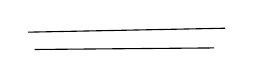
\begin{tikzpicture}\draw (0,.12)--(2.5,.17); \draw (.08,-.1)--(2.36,-.08);\end{tikzpicture}}

4) \quad Ens. de petit cardinal

a) \uline{Cardinal 2}\qquad Ens de cardinal 2 $\longleftrightarrow$ torseur \unsure{sur|sous} $\mathbb{Z}_2$ ou encore, \uline{espace affine \deleted{\unsure{sous}}} $\deleted{\unsure{\mathbb{Z}}}\mathbb{F}_2$ (ou encore, \deleted{\illegible{1}} espace affine de dim 1 sur corps $\mathbb{F}_2$ --- car les espaces vect. de dim 1 sur $\mathbb{F}_2$ sont can. isomorphes \ldots)

\[
\boxed{\operatorname{Aff}(1,\mathbb{F}_2)\simeq
 \operatorname{Aff}(\mathbb{Z}_2)\simeq\unsure{\mathfrak{S}|\mathcal{S}}_{\unsure{2|n}}}
\]
\[
(\unsure{\mathcal{A}|A}_2=\{1\})
\]

b) \uline{Cardinal 3}
\[
\begin{aligned}
\mathfrak{S}_3&\simeq\operatorname{Aff}(1,\mathbb{F}_3)&
 &\simeq\operatorname{Gl}(2,\mathbb{F}_2)&
 &\simeq\operatorname{GP}(1,\mathbb{F}_2)\\
&\hspace{2em}\rotatebox{90}{$\simeq$}&&&&\hspace{3em}\rotatebox{90}{$=$}\\
&\hspace{1em}\mathbb{F}_3^{+}\mathbin{.}\mathbb{F}_3^{*}
 &&&&\operatorname{Gl}(2,\mathbb{F}_2)/\mathbb{F}_2^{*}\\
&\hspace{1em}\rotatebox{90}{$\unsure{\simeq|=}$}
 \quad\rotatebox{90}{$=$}\\
&\hspace{.8em}\mathbb{Z}_3\quad\mathbb{Z}_2
\end{aligned}
\]
\[
\mathcal{A}_3\simeq\deleted{\unsure{\mathbb{Z}}}\mathbb{F}_3^{+}(\simeq\mathbb{Z}_3)
\]
% archive sheet number: 12

